\chapter{Traceroute}

\section{Ferramenta Traceroute}
O utilitário traceroute, que foi escrito por Van Jacobson em 1987, é uma
ferramenta de diagnóstico que nos permite ver a rota que datagramas IP seguem
 quando são enviados de um host a outro.

Seu funcionamento está baseado no uso do campo Time to Live (TTL) do pacote IPv4
destinado a limitar o tempo de vida dele. Este valor é decrementado a cada vez
que o pacote é encaminhado por um roteador. Ao atingir o valor zero o pacote é
descartado e o originador é alertado por uma mensagem ICMP TIME EXCEEDED.
Através da manipulação do campo TTL de uma série de datagramas UDP é possível
receber esta mensagem de cada um dos roteadores no caminho do pacote. Para
o caso do IPv6 é utilizado o campo hop limit, o limite de saltos dos
datagramas desta versão do protocolo. A implementação disponível no
Microsoft Windows utiliza apenas pacotes ICMP.

O traceroute envia um datagrama com um TTL igual a 1 ao host de destino.
Ao chegar ao primeiro rotador no caminho, o TTL é decrementado, ficando
com o valor zero, de modo que o datagrama é descartado e a mensagem ICMP
“Tempo Excedido” é enviada de volta à origem. Desta forma, o primeiro roteador
no caminho é identificado. Então, o traceroute envia um novo datagrama, desta
vez com o TTL igual a 2, que passará pelo primeiro roteador, que decrementa o
TTL para 1, e então será descartado no segundo roteador e assim, descobrimos
o endereço IP deste roteador também. Esse processo continua até que um datagrama
 chegue ao host de destino.


Porém, ao chegar no host de destino, mesmo que o TTL do datagrama seja igual a 1,
ele não será descartado e, portanto, a mensagem ICMP Tempo Excedido não será gerada.
Neste caso, como sabemos que o pacote chegou a seu destino? Isso vai depender do
sistema operacional utilizado (mais precisamente, do utilitário presente); No Unix
e derivados, o traceroute envia pacotes UDP, escolhendo portas de um valor elevado,
que muito provavelmente não são utilizadas por nenhuma aplicação no host de destino.
Desta forma, o host de destino gerará um erro ICMP do tipo “Porta Inalcançável” – e,
então, tudo o que o traceroute tem a fazer é diferenciar o recebimento de mensagens
Tempo Excedido da mensagem Porta Inalcançável para saber quando parar.

\section{Experimento}

Na terceira parte do segundo problema deste trabalho devemos realizar os testes
utilizando o traceroute como ferramenta para diagnóstico de rede,
além disso utilizaremos o wireshark como ferramenta de captura de pacotes,
todos os testes deste experimento foram feitos utilizando:

\begin{itemize}
  \item[linux:] Linux debian jessie, kernel 4.1.0-2-amd64
  \item[wireshark] Wireshark 1.12.8
  \item[traceroute] 2.0.21
\end{itemize}

Para preparar o wireshark devemos selecionar uma interface de rede para monitorar,
para fazer isto basta ir ao menu superior na opção capture -> iterfaces, ou
pelo atalho ctrl +i.

\begin{figure}[h]
  \centering
  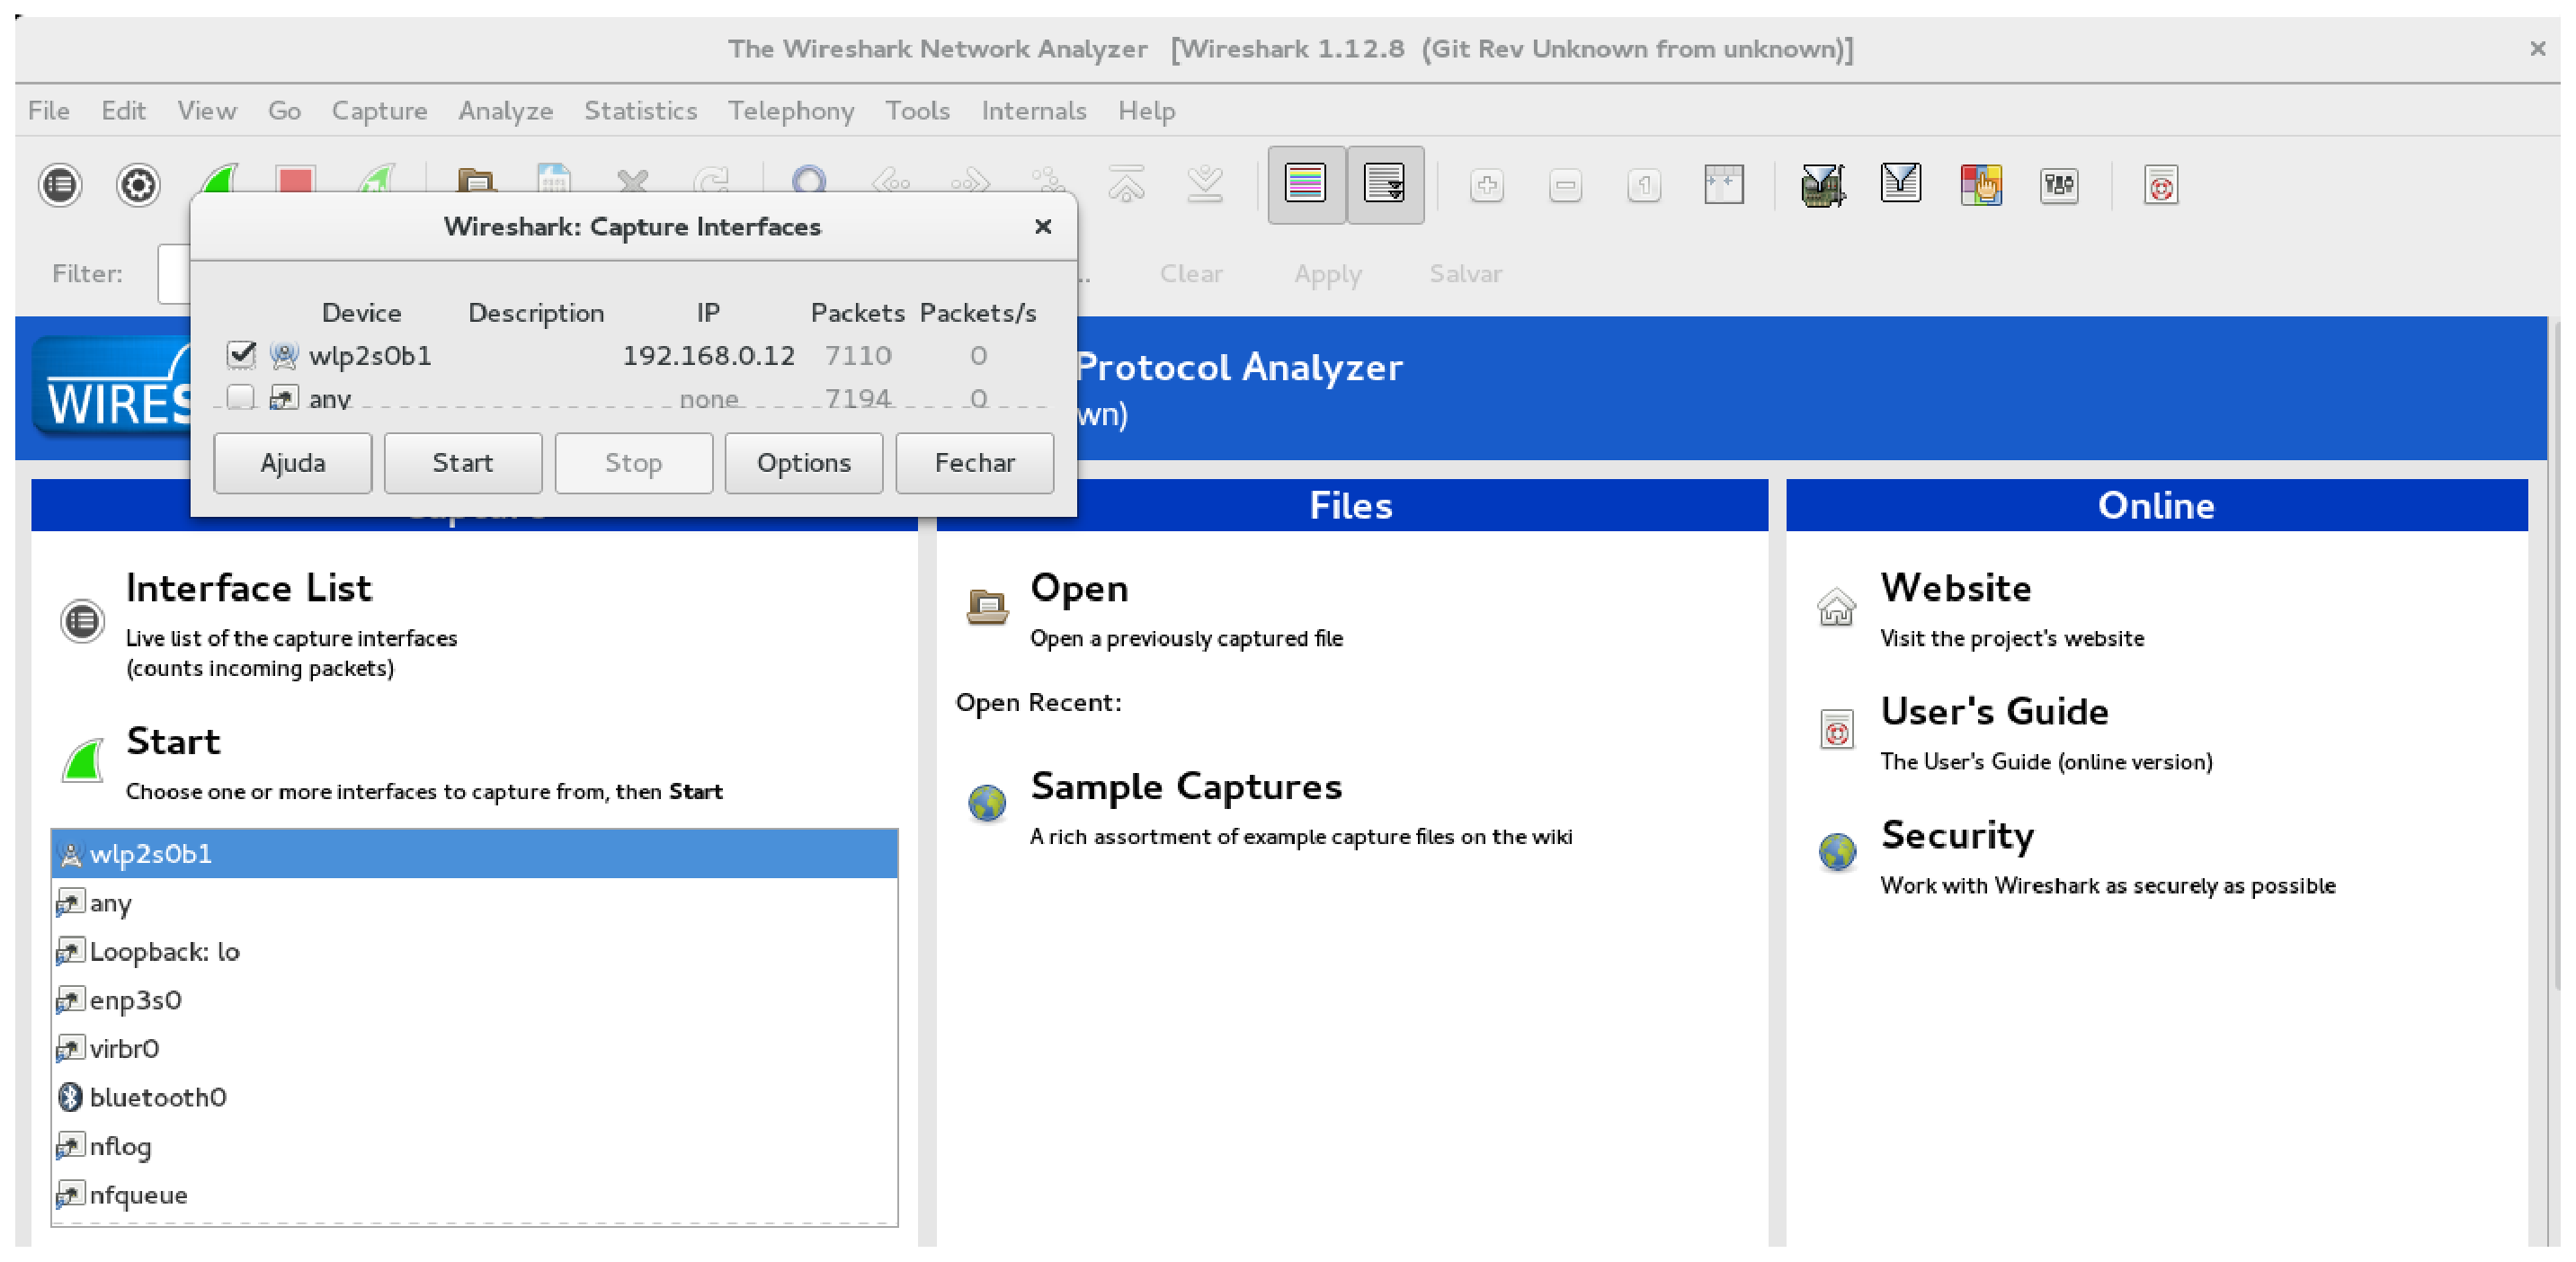
\includegraphics[width=0.9\textwidth]{figuras/f1.eps}
  \caption{Configurando wireshark}
  \label{fig:f1}
\end{figure}


Após clicar em start a rede começa a ser monitorada como, por exemplo,
na rede escolhida podemos ver a comunicação entre os dispositivos que estão
conectados na rede e o roteador.

\begin{figure}[h]
  \centering
  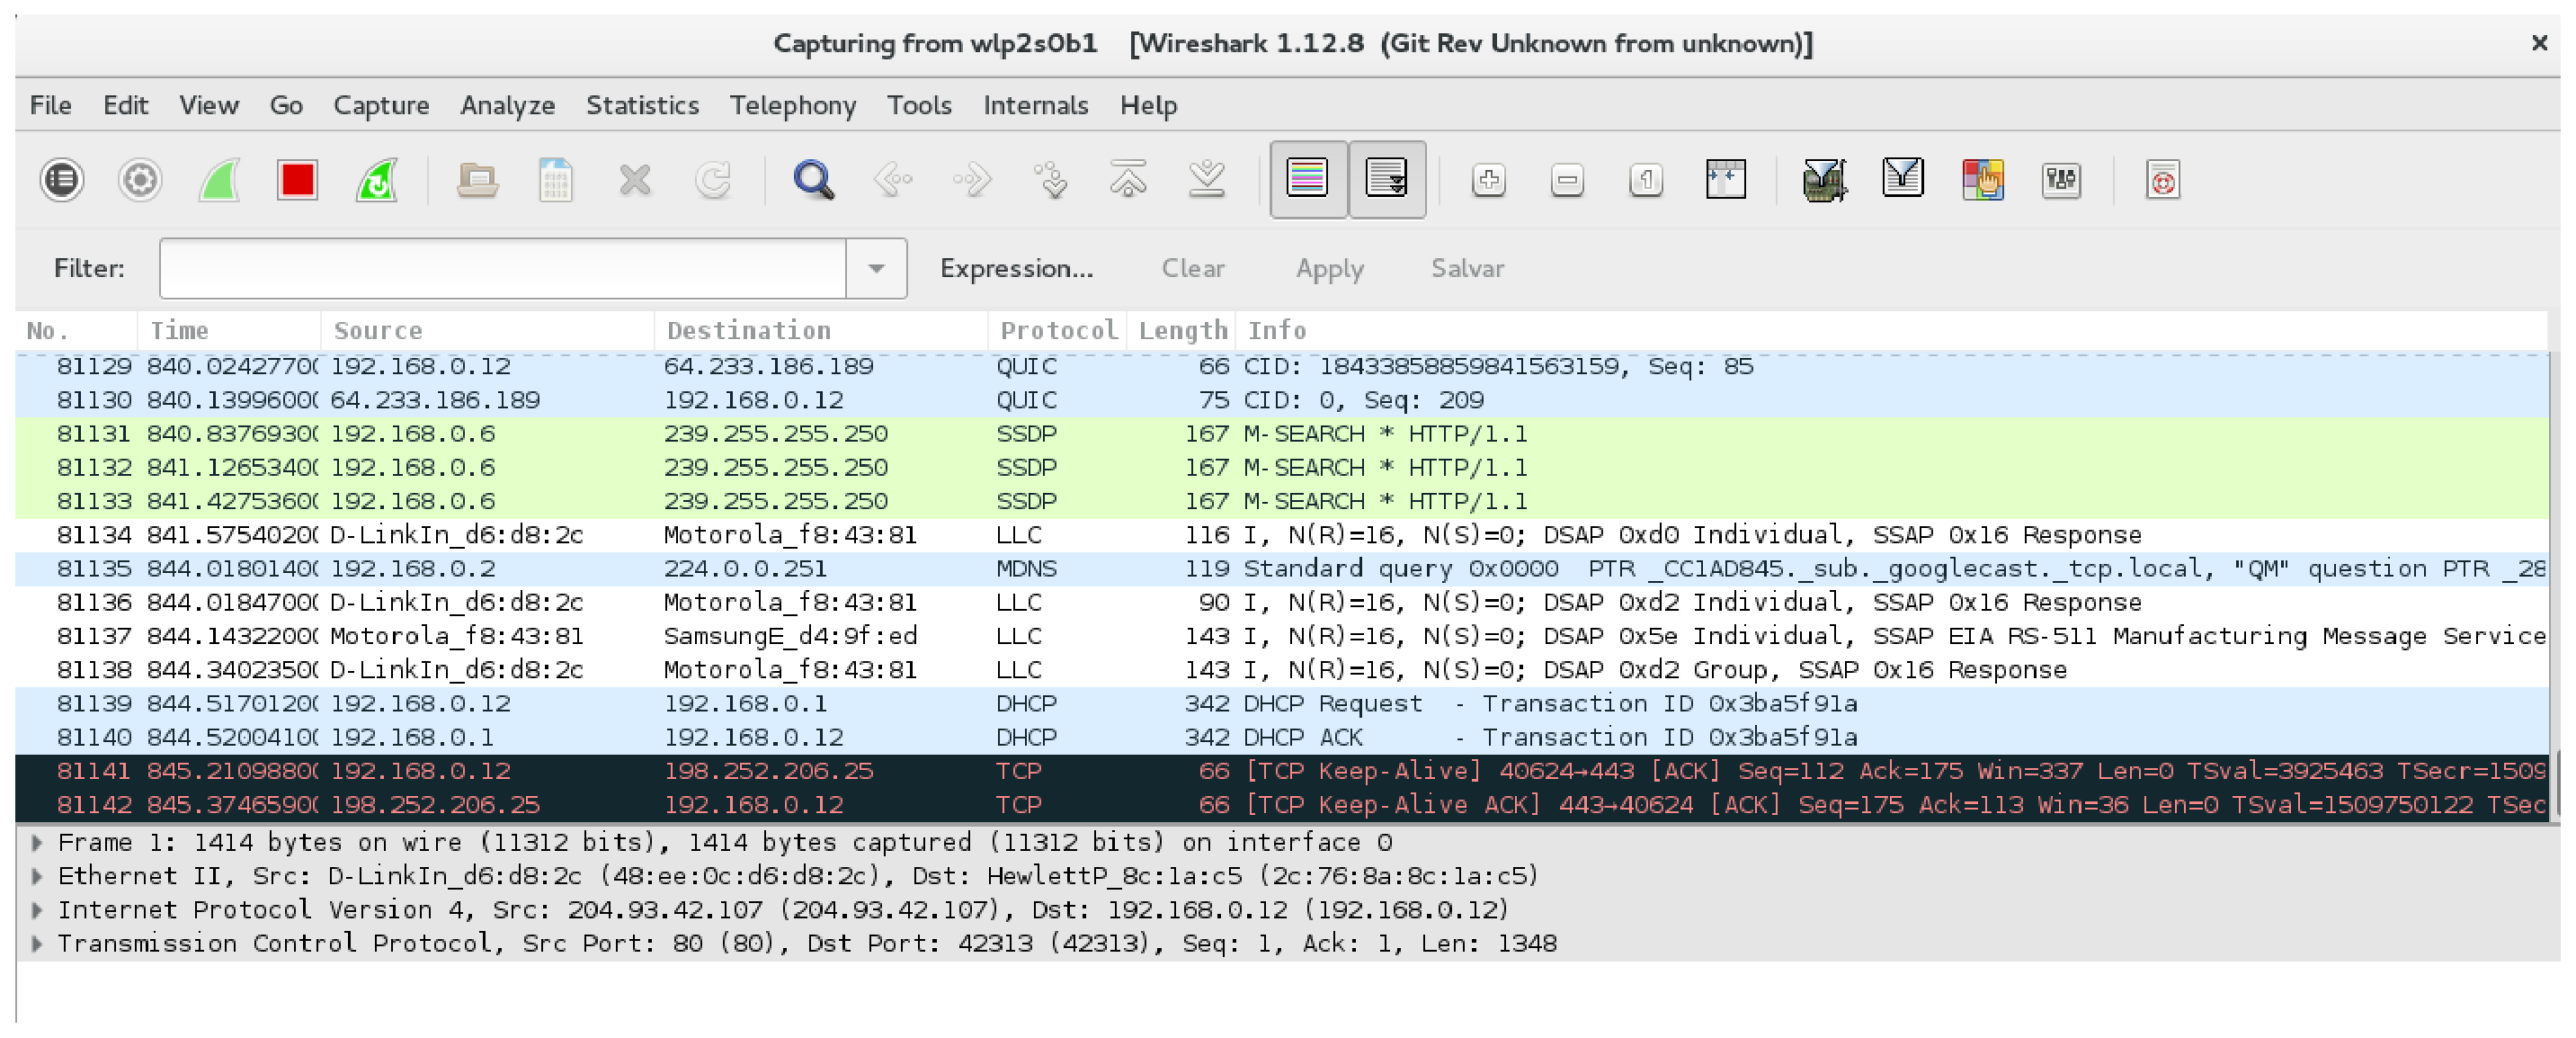
\includegraphics[width=0.9\textwidth]{figuras/f2.eps}
  \caption{Wireshark}
  \label{fig:f2}
\end{figure}


Agora vamos acompanhar o traceroute, para nosso teste vamos apontar nosso
traceroute para gmail.com, após acompanhar o traceroute vamos analisar os
pacotes com o wireshark. Ao executar o comando traceroute gmail.com se obtêm:

\begin{figure}[h]
  \centering
  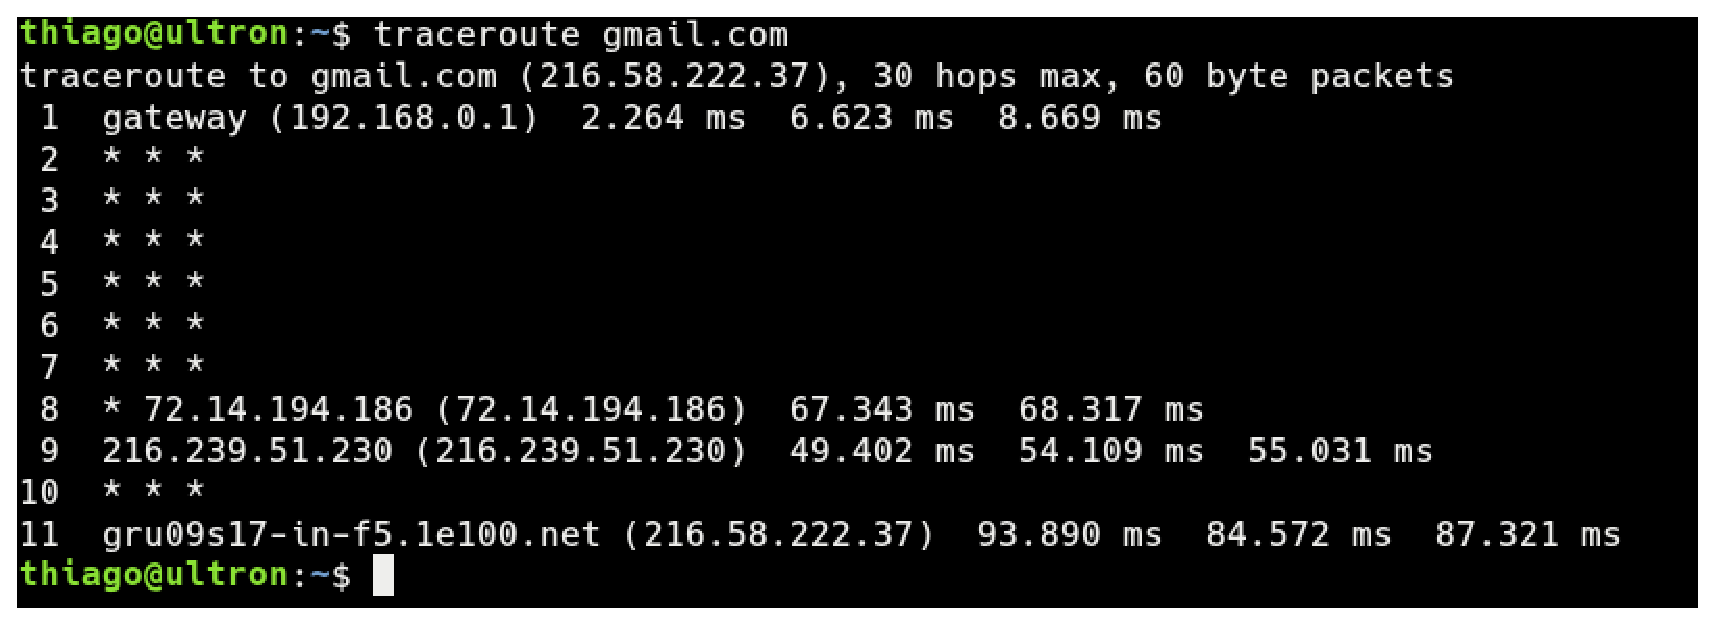
\includegraphics[width=0.9\textwidth]{figuras/f3.eps}
  \caption{Traceroute}
  \label{fig:f3}
\end{figure}

Nota-se que foram enviados pacotes de 60 bytes de tamanho e 30 hops (saltos) no
máximo. O primeiro gateway encontrado é o gateway do roteador da rede de origem,
os * indicam que não houve resposta naquele ponto em um período de 5 segundos.
Isso pode ocorrer por alguns motivos como problemas na rede, firewals que filtram
portas UDP, etc.

Após usar o traceroute com o wireshark capturando os pacotes da rede podemos fazer
um relatório do que de fato aconteceu e comparar com a teoria da disciplina de
fundamento de redes abordando os tópicos sugeridos no roteiro deste trabalho.

Como vimos, o primeiro trabalho que o traceroute precisa fazer é descobrir o
endereço ip do nome www.gmail.com, com isso seria necessário fazer uma consulta
ao servidor de DNS, como podemos ver no wireshark :

\begin{figure}[h]
  \centering
  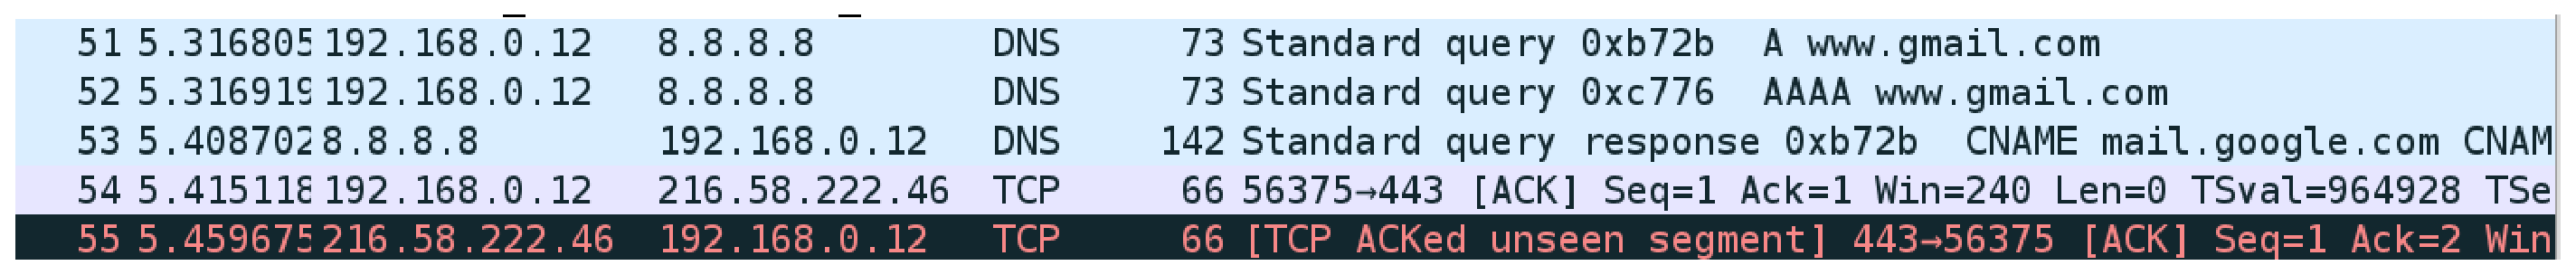
\includegraphics[width=0.9\textwidth]{figuras/f4.eps}
  \caption{Captura com wireshark}
  \label{fig:f4}
\end{figure}

O endereço do host de origem (chamaremos de H1) é 192.168.0.12 e ela manda um
pacote para o servidor DNS ( 8.8.8.8), logo em seguida o servidor DNS devolve
a H1 a resposta da consulta, utilizando o recurso do wireshark podemos ver
detalhadamente essa informação:

\begin{figure}[h]
  \centering
  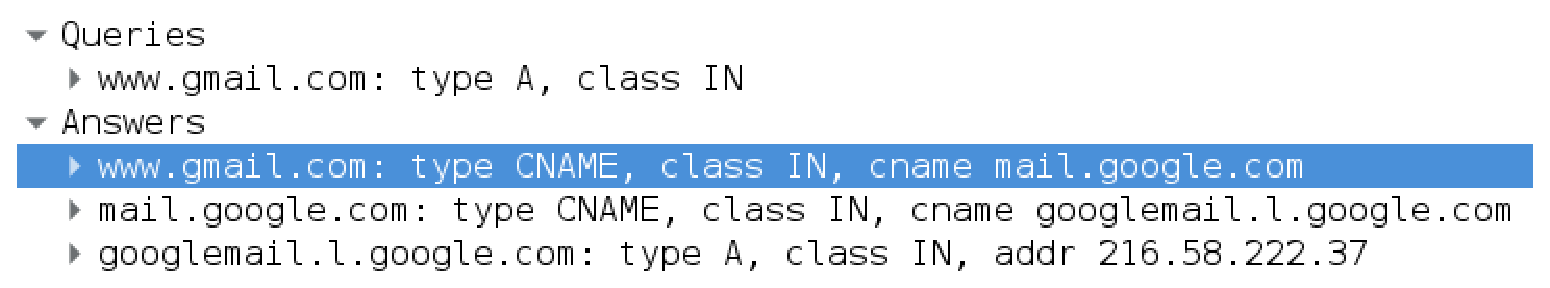
\includegraphics[width=0.9\textwidth]{figuras/f5.eps}
  \caption{Captura de dns com wireshark}
  \label{fig:f5}
\end{figure}

Podemos ver que o servidor DNS que utiliza segmentos UDP responde o IP após
resolver a consulta www.gmail.com. Com o ip 216.58.222.37 em mãos agora podemos
 ver os segmentos UDP que o traceroute deve enviar, como vimos na parte teórica.
Analisando agora os segmentos enviados de H1 até o destino 216.58.222.37 que
chamaremos de D1, percebemos que alguns pacotes não chegaram, como, por exemplo:

\begin{figure}[h]
  \centering
  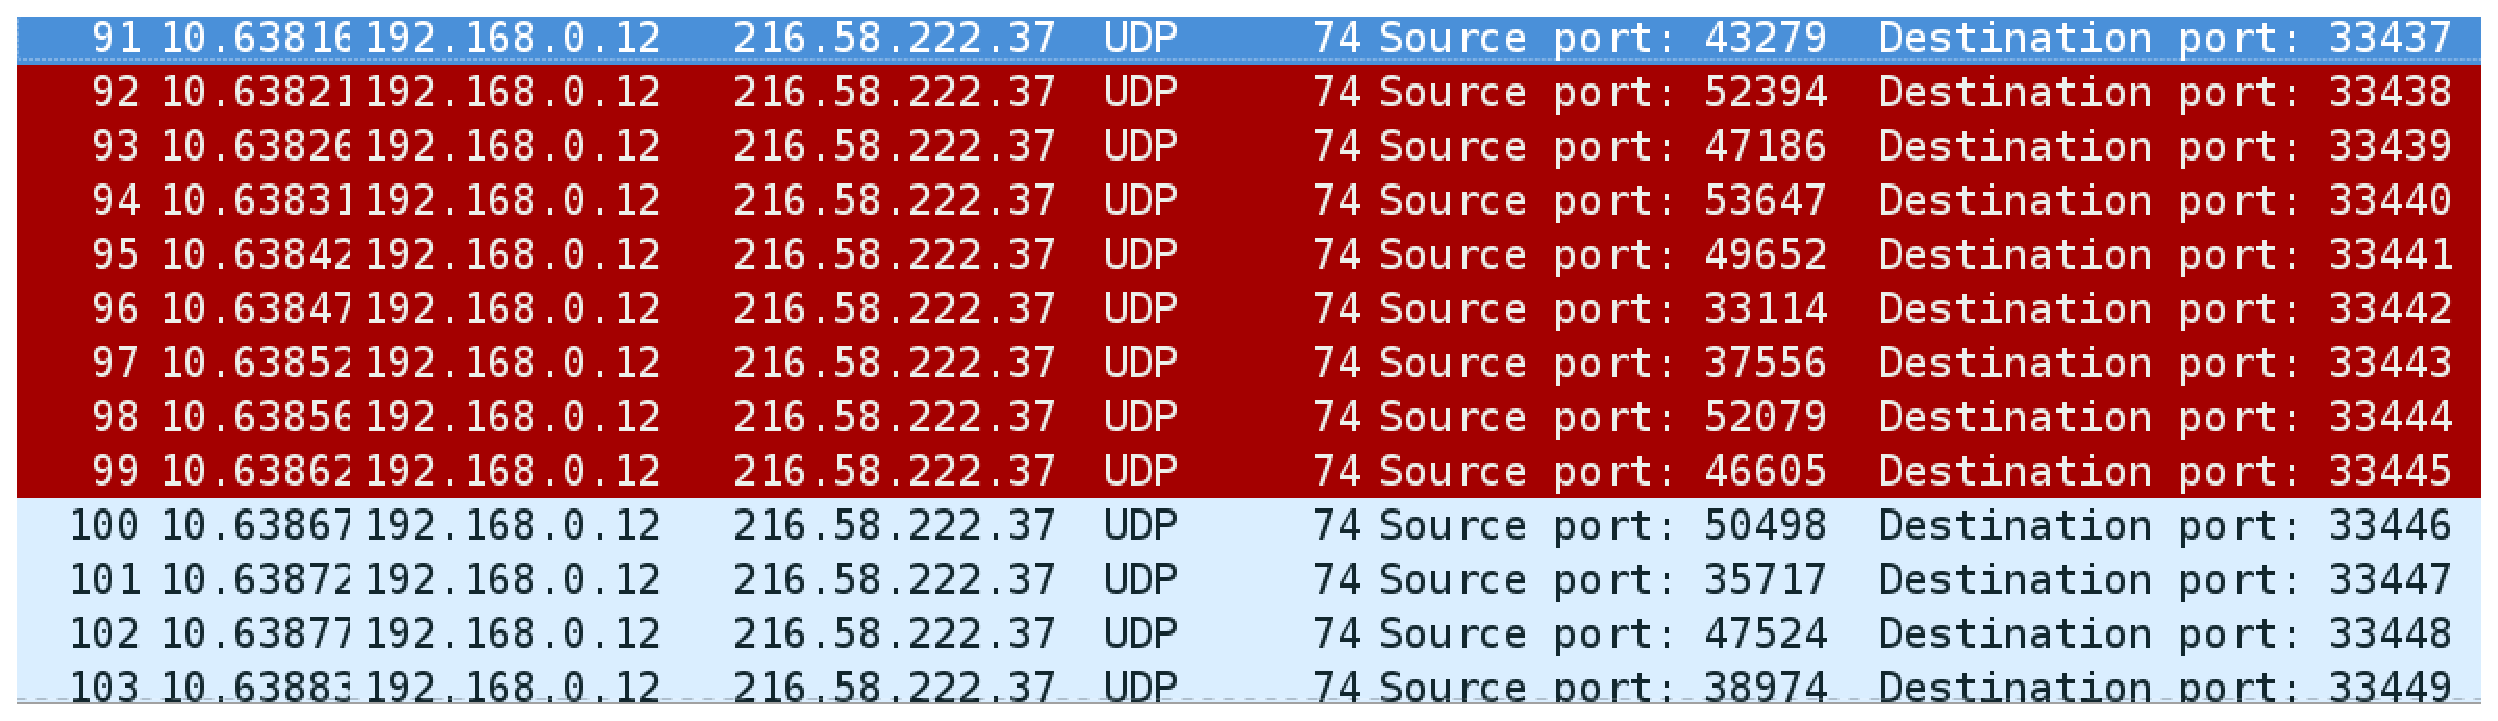
\includegraphics[width=0.9\textwidth]{figuras/f6.eps}
  \caption{Captura de pacotes com wireshark}
  \label{fig:f6}
\end{figure}

Um dos motivos pode ser que o firewall pode estar bloqueando acesso a algumas
portas, vimos também que o traceroute envia segmentos UDP em portas altas e
aleatórias. Outros segmentos conseguem chegar, como esperado, D1 devolve a H1
pelo protocolo ICMP um pacote com Destination enrechable (port unrechable)
referente aos pacotes perdidos, como podemos ver no wireshark:

\begin{figure}[h]
  \centering
  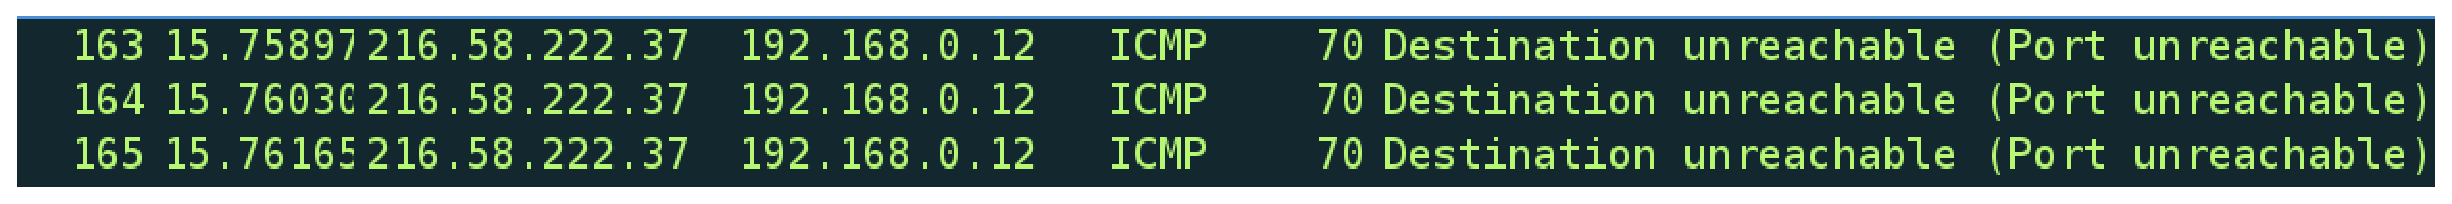
\includegraphics[width=0.9\textwidth]{figuras/f7.eps}
  \caption{Captura de pacotes com wireshark}
  \label{fig:f7}
\end{figure}

Também temos o caso dos  asterísticos imprimidos pelo traceroute, que nada mais
é do que os pacotes que extrapolaram o tempo de vida, com isso como esperado, o
roteador 192.168.0.1 devolve a H1 pelo protocolo ICMP um pacote com TIme To
Live Exceeded in transmit, como podemos ver no wireshark:

\begin{figure}[h]
  \centering
  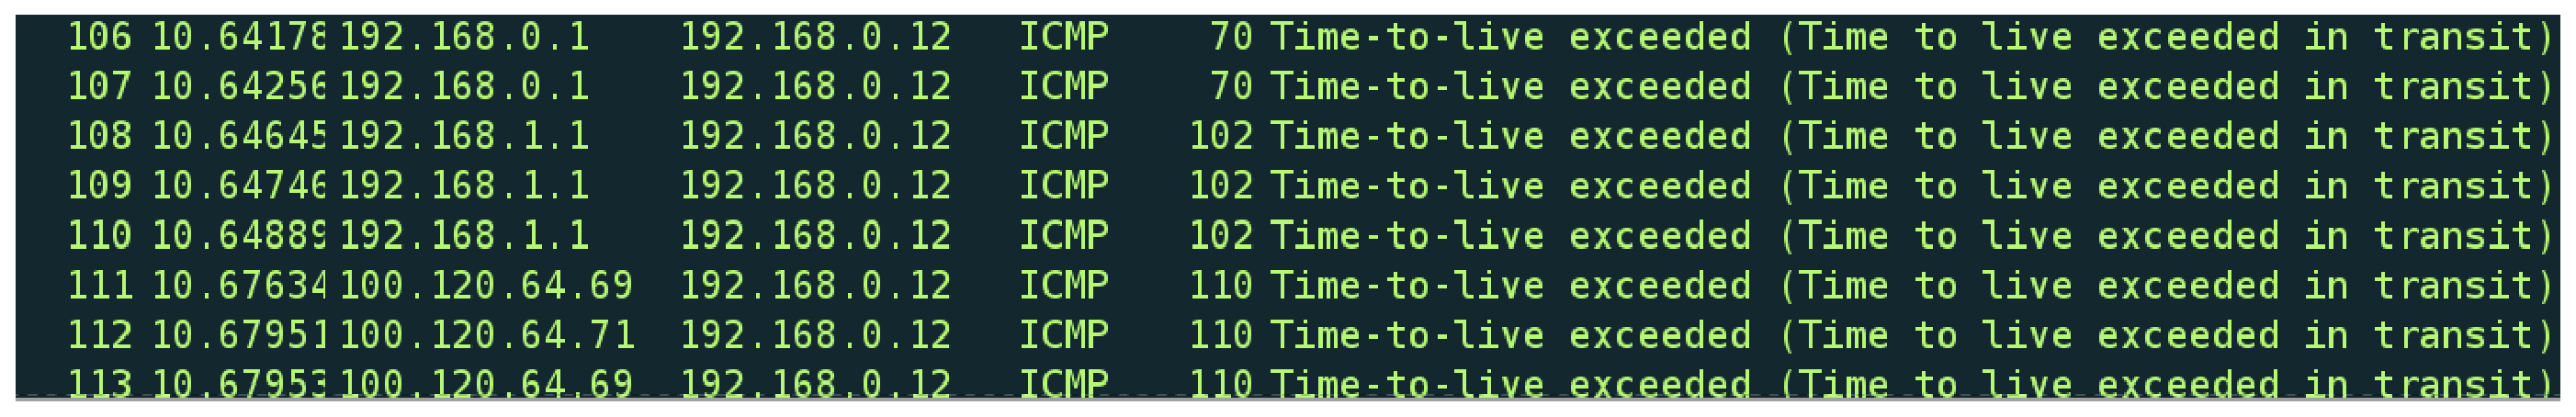
\includegraphics[width=0.9\textwidth]{figuras/f8.eps}
  \caption{Captura de pacotes com wireshark}
  \label{fig:f8}
\end{figure}

Isso acontece pelo fato de que a cada vez que o pacote não chega ao destino
seu tempo de vida é aumentado por uma unidade como, por exemplo, na imagem abaixo:

\begin{figure}[h]
  \centering
  \includegraphics[width=0.9\textwidth]{figuras/f9.eps}
  \caption{Funcionamento do traceroute}
  \label{fig:f9}
\end{figure}

Por fim, quando o pacote consegue chegar a origem sem receber TTL excedido
consegue-se finalmente atingir o endereço ip do gmail.com conhecido no
início deste experimento.

Durante o experimento notou-se algo curioso, notamos que os pacotes que chegavam
em D1 até H1 possuem um protocolo diferente em relação ao UDP, o chamado QUIC
(Quick UDP Internet Connections), desenvolvido pela google a partir de 2012 e
iniciou-se os experimentos a partir de 2013. QUIC suporta um conjunto de conexões
multiplexados entre dois pontos de extremidade UDP, e foi projetado para fornecer
proteção de segurança equivalente a TLS / SSL, juntamente com conexão reduzida e
latência de transporte, e estimativa de largura de banda em cada direção para
evitar o congestionamento. O objetivo de longo prazo para o Google, QUIC
pretende ser quase equivalente a uma conexão TCP independente, mas com muito
menor latência.

\begin{figure}[h]
  \centering
  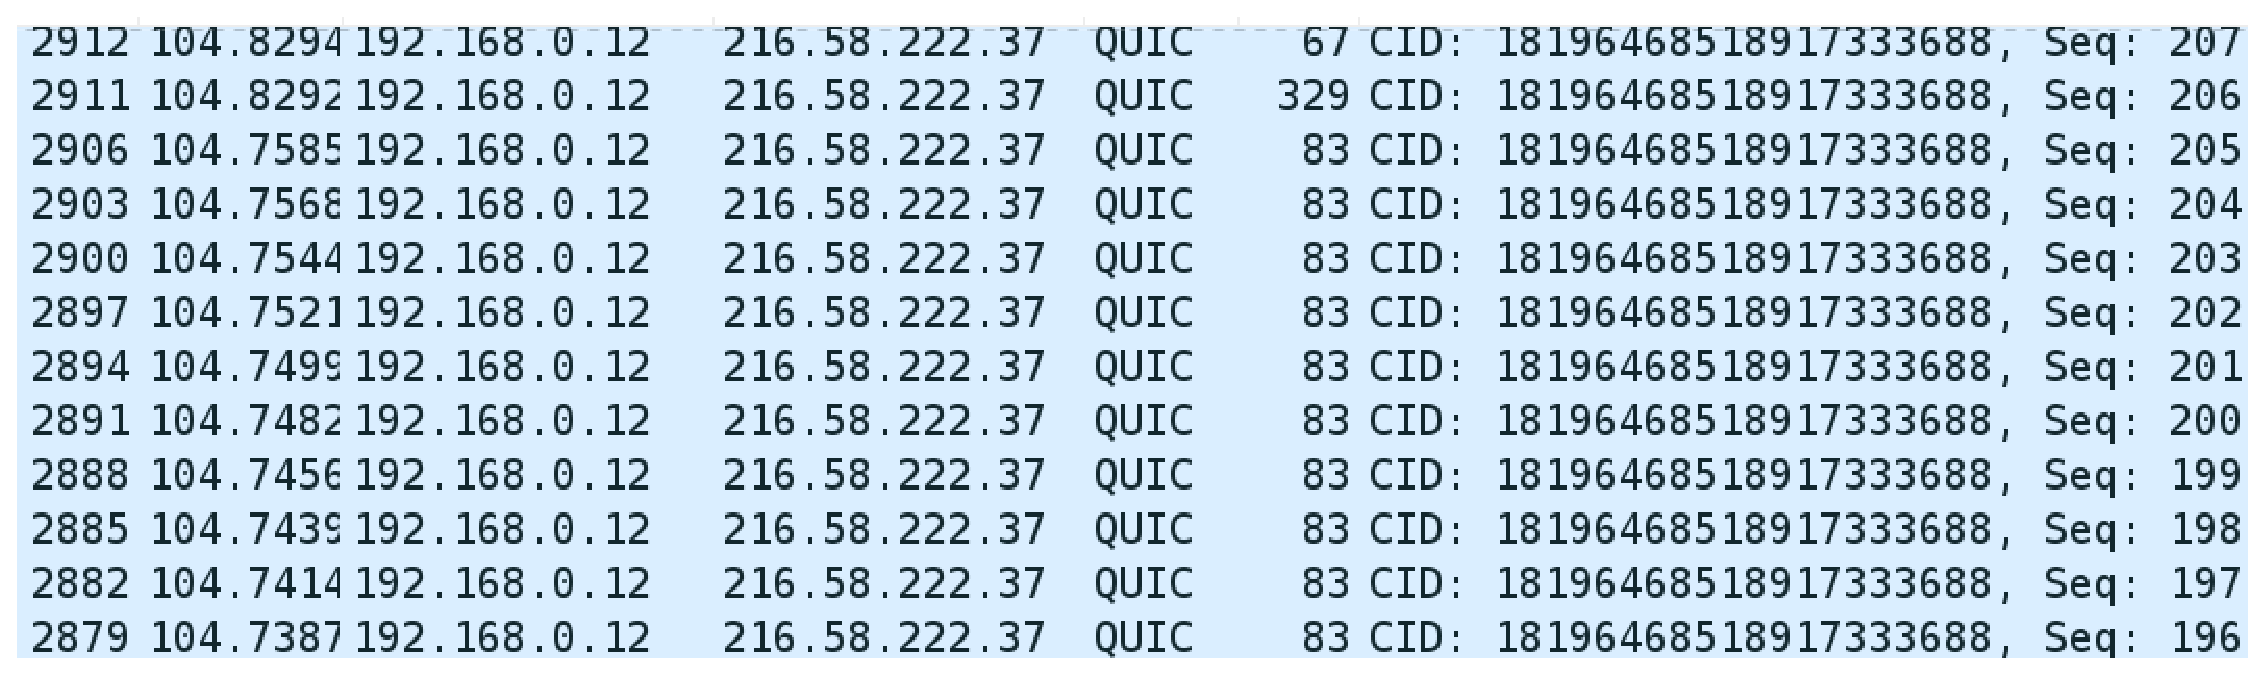
\includegraphics[width=0.9\textwidth]{figuras/f10.eps}
  \caption{Captura de pacotes com wireshark}
  \label{fig:f10}
\end{figure}

Uma outra curiosidade no experimento é que também encontramos segmentos com
protocolo TLS v1 que é um protocolo de segurança de proteção para serviços de email.
